\subsection{Small Signal}

Figure \ref{fig:Sac120} shows the gain and phase at various common mode voltages.
It shows clearly that the DC gain of $60dB$ is met, it is still at approximately the same value at $100KHz$ and is therefore much greater than the required $26dB$.

\begin{figure}[H]
	\centering
	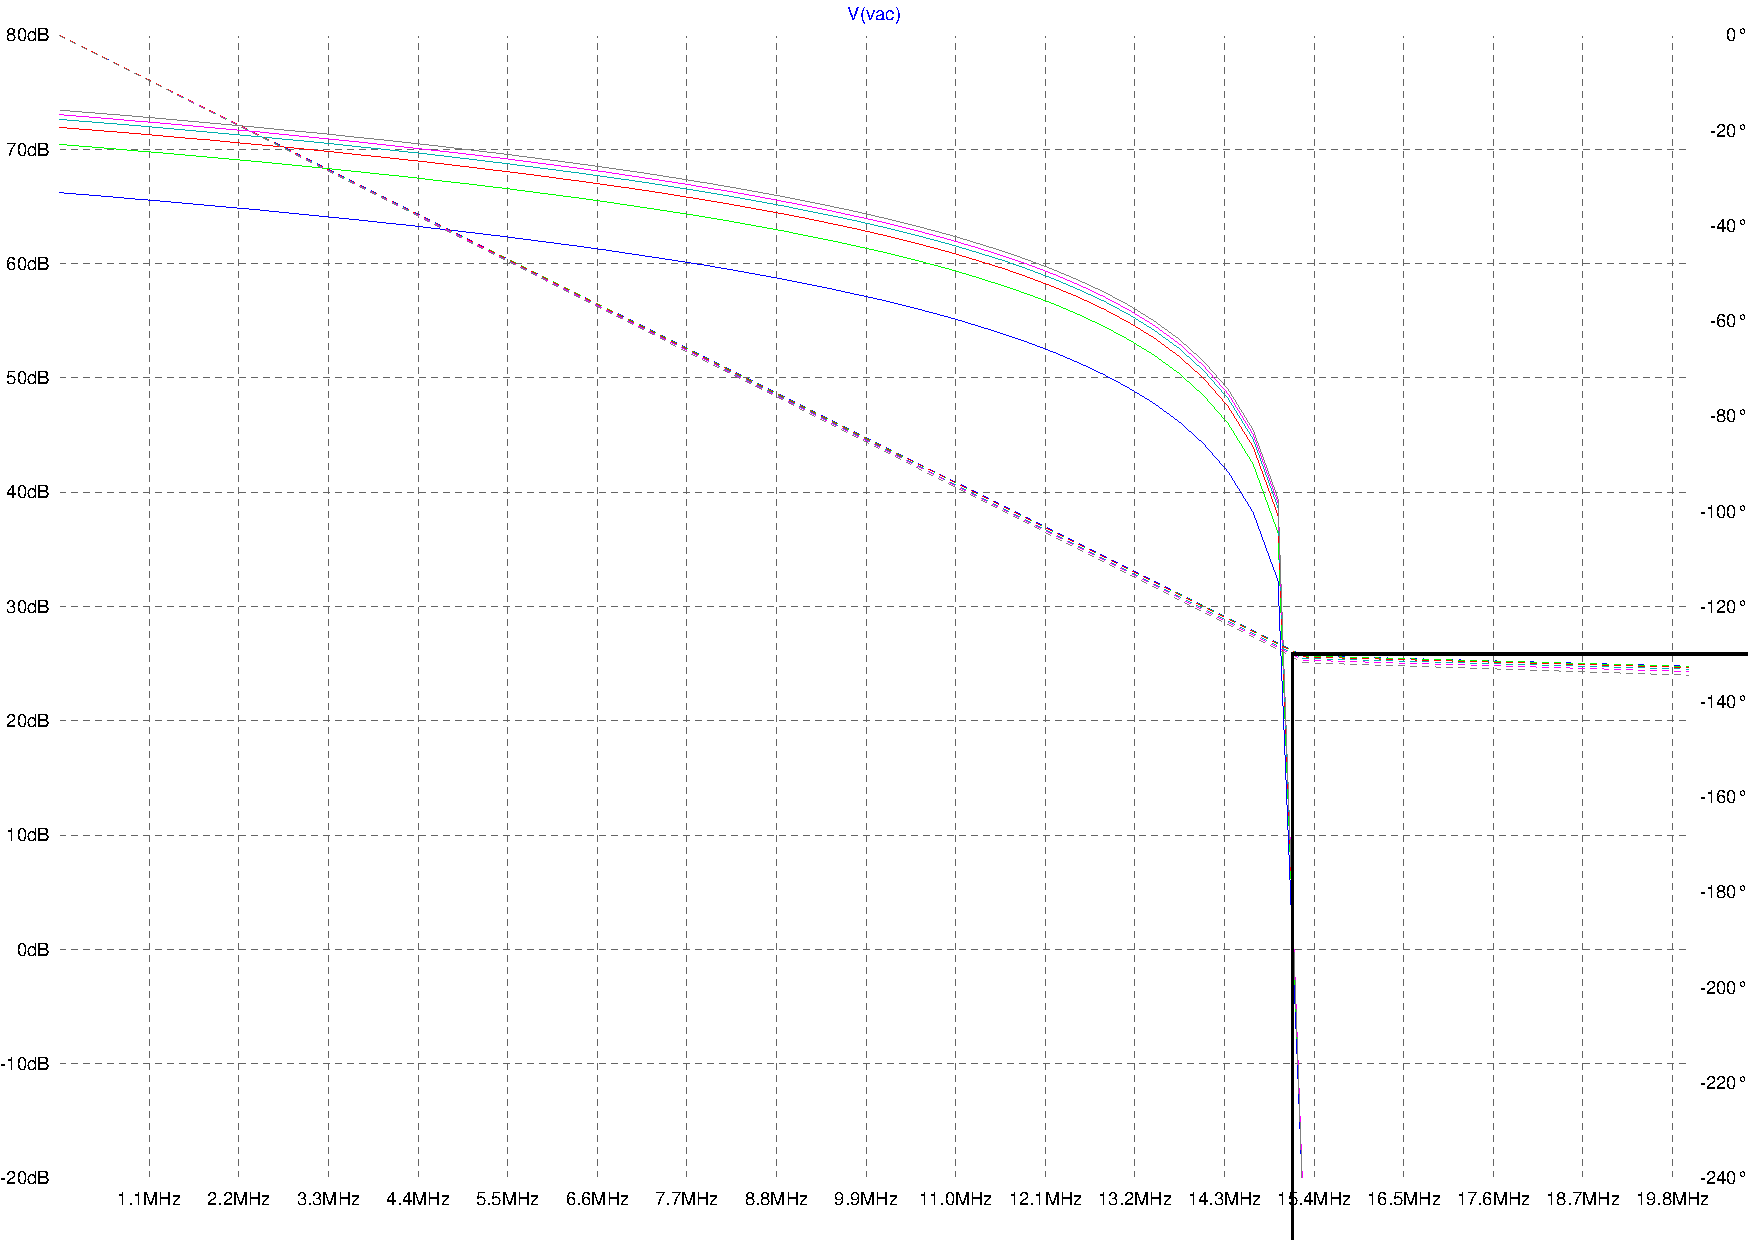
\includegraphics[width=\textwidth]{./images/BasicAC-multi.pdf}
	\caption{The gain and phase of the device for common mode levels $0.3V$, $0.4V$, $0.5V$, $0.6V$, $0.7V$, and $0.8V$, all with a $C_{L} = 120pF$}
	\label{fig:Sac120}
\end{figure}

The phase at unity gain can be seen to be approximately $-128^{\circ}$.
This results in a phase margin of: \\
$\phi_{120pF} = 180^{\circ} - 128^{\circ}$ \\
$\phi_{120pF} = 52^{\circ}$ \\
This is greater than the required $45^{\circ}$, and is therefore within specification.

\begin{figure}[H]
	\centering
	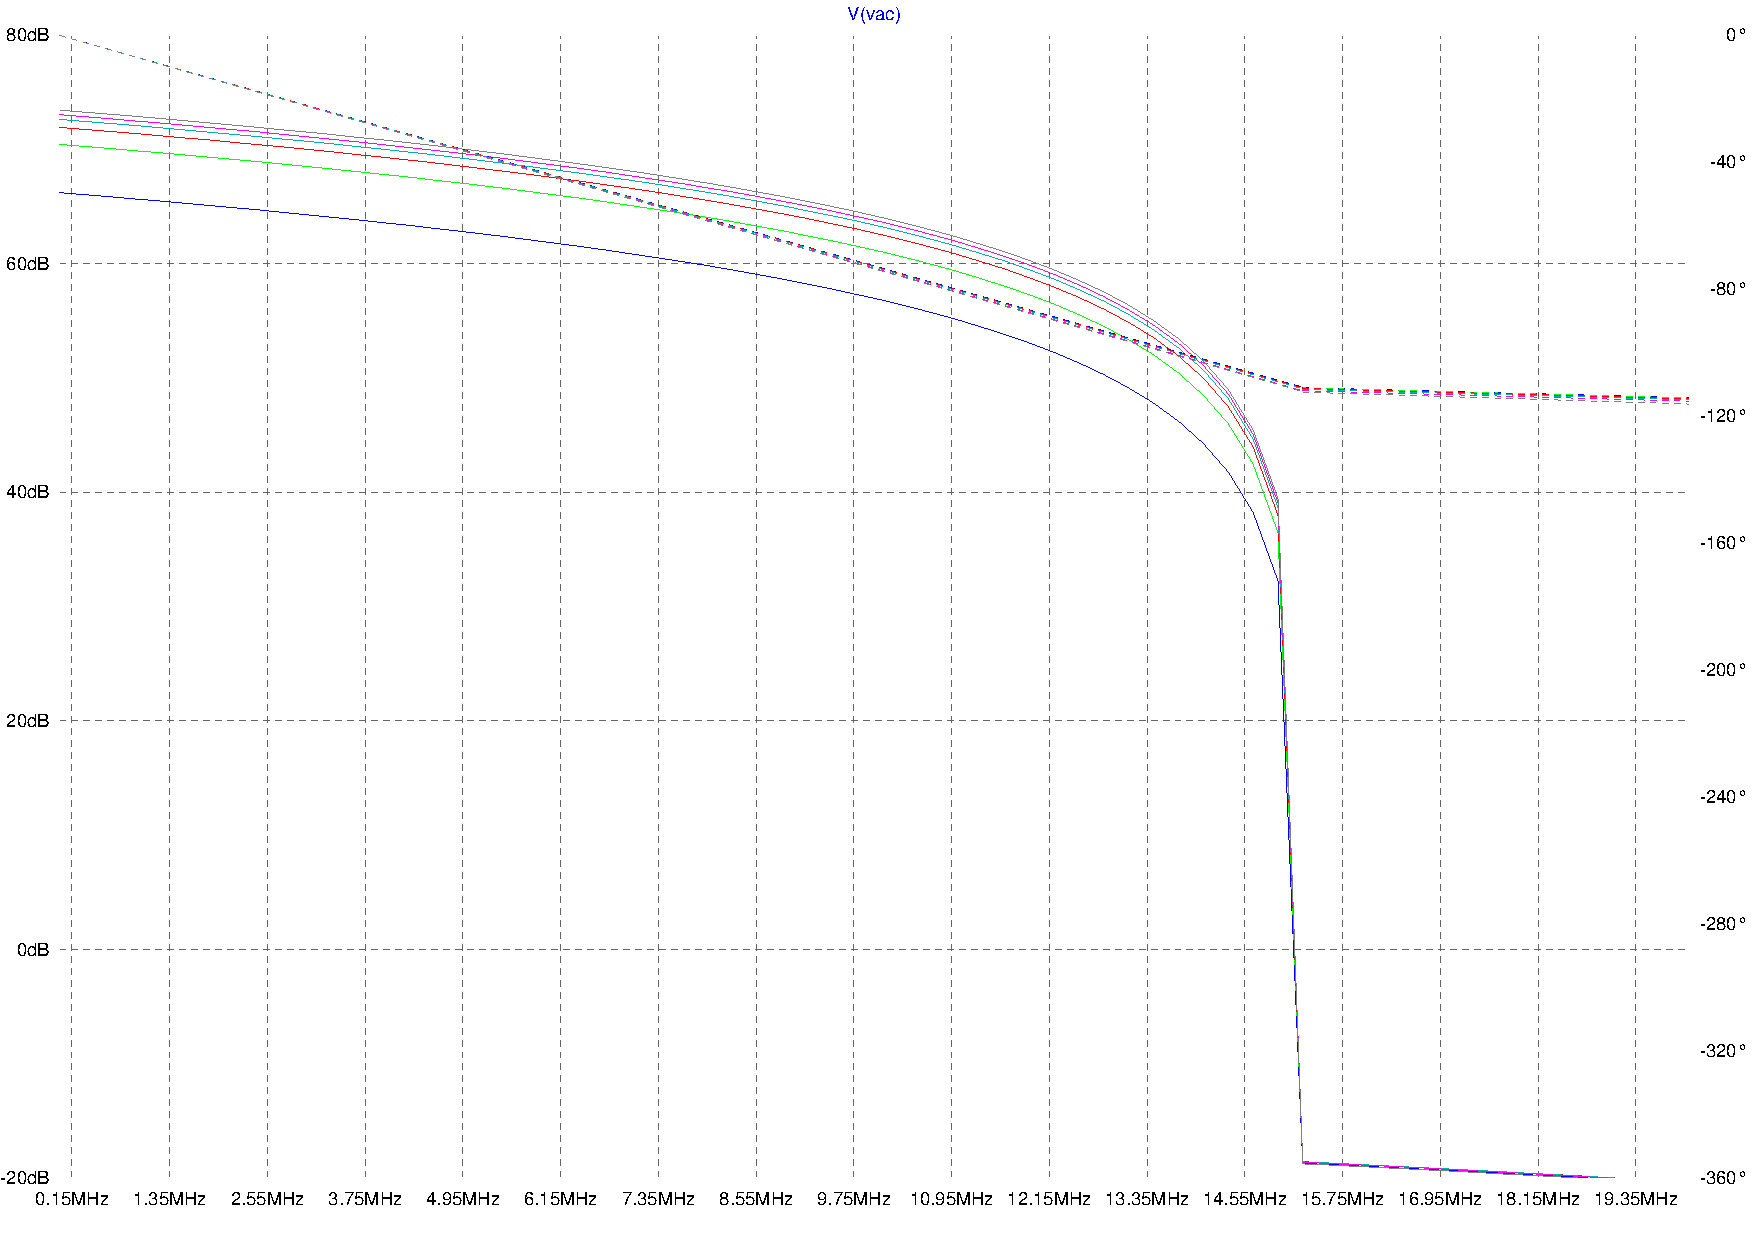
\includegraphics[width=\textwidth]{./images/BasicAC-multi-60.pdf}
	\caption{The gain and phase of the device for common mode levels $0.3V$, $0.4V$, $0.5V$, $0.6V$, $0.7V$, and $0.8V$, all with a $C_{L} = 60pF$}
	\label{fig:Sac60}
\end{figure}

In this diagram the DC gain reaches as low as about $68dB$, which is above the $60dB$ requirement.
The phase margin here is:
$\phi_{60pF} = 180^{\circ} - 110^{\circ}$ \\
$\phi_{60pF} = 70^{\circ}$ \\
This is greater than the required $45^{\circ}$, and is therefore within specification.

\begin{figure}[H]
	\centering
	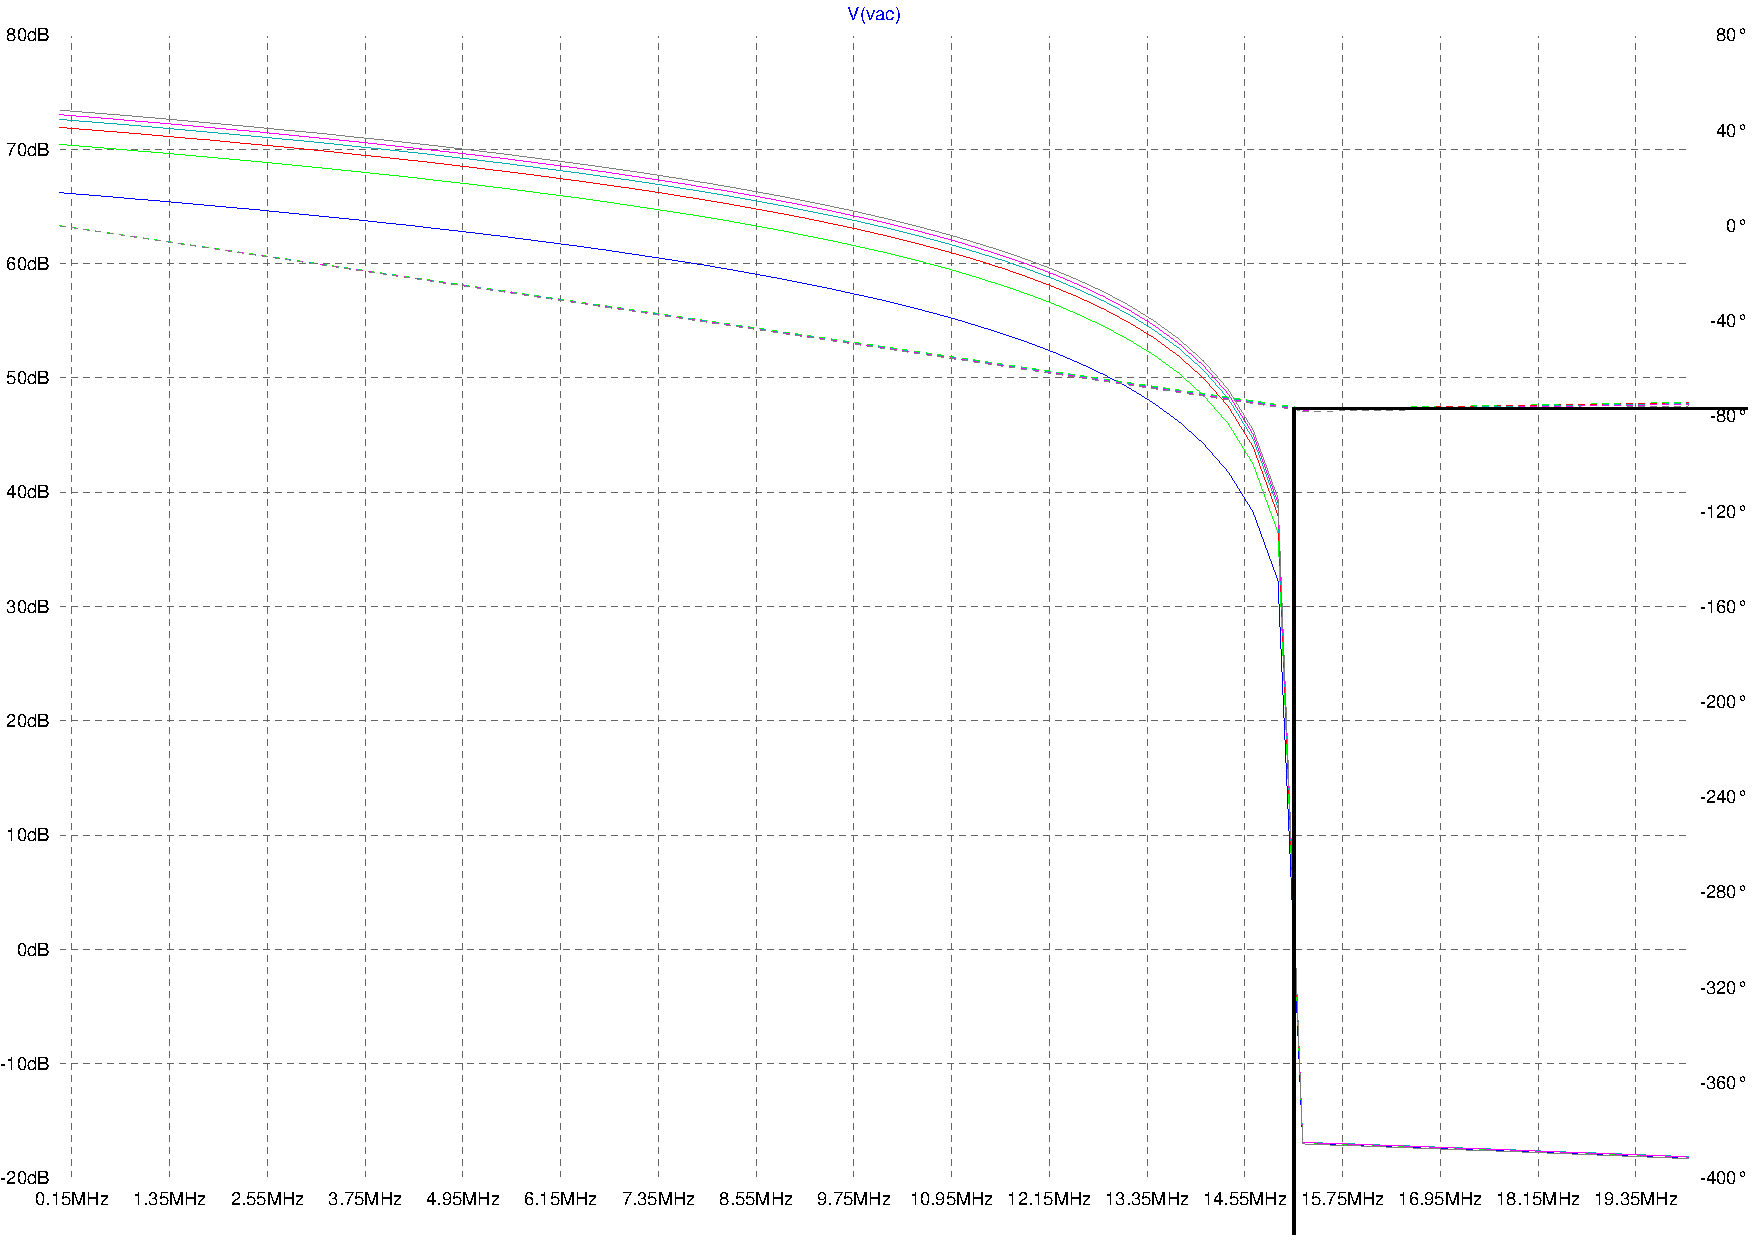
\includegraphics[width=\textwidth]{./images/BasicAC-multi-0.pdf}
	\caption{The gain and phase of the device for common mode levels $0.3V$, $0.4V$, $0.5V$, $0.6V$, $0.7V$, and $0.8V$, all with a $C_{L} = 0pF$}
	\label{fig:Sac0}
\end{figure}

In this diagram the DC gain reaches as low as about $66dB$, which is above the $60dB$ requirement.
The phase margin here is:
$\phi_{60pF} = 180^{\circ} - 75^{\circ}$ \\
$\phi_{60pF} = 105^{\circ}$ \\
This is greater than the required $45^{\circ}$, and is therefore within specification.


